\documentclass[12pt,a4paper]{article}
\usepackage[italian]{babel}
\usepackage[T1]{fontenc}
\usepackage[utf8x]{inputenc}
\usepackage{graphicx}
\graphicspath{{images/}}

\begin{document}

\title{Tesi}
\author{Davide Malvezzi}
\date{2017/2018}
\maketitle
\newpage

\tableofcontents
\newpage

\section{Introduzione}
\subsection{Cos'è Eco-Marathon?}
L’Eco-Marathon è una competizione annuale organizzata dalla Shell nella quale team di studenti e professori, universitari e di scuole superiori di tutta Europa, gareggiano con veicoli speciali cercando di portare a termine un numero prefissato di giri di pista con il minor consumo di energia possibile. 
Questa competizione nacque nel 1939 negli Stati Uniti dalla scommessa di due ingegneri della Shell, che si sfidarono a coprire con i propri veicoli la maggior distanza possibile con un solo litro di benzina. L’Eco-Marathon, nella sua forma attuale, si svolse per la prima volta in Francia nel 1985 e alla quale partecipano tuttora più di 200 team all’anno. I veicoli partecipanti sono divisi in due categorie: i Prototipi, che puntano alla massima efficienza tralasciando il comfort dei passeggeri, e le UrbanConcept, realizzate per assomigliare alle auto per uso urbano. 
I veicoli sono anche divisi in base alla tipologia di energia utilizzata:
veicoli con motore a combustione interna utilizzano benzina, diesel o etanolo;
veicoli elettrici utilizzano celle a idrogeno o batterie al litio.
L’evento ha luogo solitamente in un autodromo, dove per alcuni giorni ogni team ha a disposizione un numero prestabilito di tentativi, solitamente quattro, per ottenere la miglior prestazione possibile. Alla fine di queste giornate gli organizzatori nominano un vincitore per ogni categoria e per ogni fonte di energia utilizzata. Vengono anche assegnati premi per il design, l’innovazione tecnologica e il lavoro di squadra. Ovviamente esiste un insieme di regole che tutti i team devono rispettare per lo svolgimento in sicurezza dell’evento, ma che incoraggiano anche i team a provare soluzioni sempre nuove. Lo spirito dell’Eco-Marathon è basato sull’innovazione, la creatività e la condivisione di esperienze ed idee fra i vari team che potranno fornire nuovi risultati e stimoli per innovazioni future.
\newpage

\subsection{Cos'è Escorpio?}
Escorpio è il nome del prototipo con il quale il Team ZeroC dell’Istituto Tecnico Industriale Leonardo da Vinci di Carpi partecipa da oltre 10 anni alla Shell Eco-Marathon. Il team nasce nel 2007 per opera dei professori Stefano Covezzi e Marco Vidoni che per caso scoprirono l’iniziativa proposta dalla Shell. Da qui nacque il Team ZeroC, composto principalmente da studenti di meccanica ed elettronica, e il veicolo Escorpio, il cui nome deriva da un’invenzione di Leonardo da Vinci. Fino al 2012 il team si è occupato della progettazione e della realizzazione del veicolo elettrico alimentato attraverso una fuel-cell a idrogeno. 
Dal 2013 il team ha deciso di abbandonare l’alimentazione a idrogeno a causa degli elevati costi delle fuel-cell per sperimentare un veicolo ibrido alimentato da una batteria agli ioni di litio e ricaricata da un pannello fotovoltaico, posto sopra la scocca del prototipo. I risultati furono ottimi e il team riuscì ad essere nella top ten per due anni di fila nella categoria veicoli elettrici.
Pur non avendo brillato nelle prestazioni, a causa di una fuoriuscita di idrogeno dalla fuel-cell, orgoglio del team è la vittoria dell’ambito Technical Innovation Award, premio per l’innovazione tecnologica, ottenuto nel 2012 grazie ad un sistema di super condensatori che permetteva di livellare il carico di potenza assorbita sulla fuel-cell, ottimizzandone i consumi. 
Il team condivide pienamente gli ideali proposti da questa iniziativa e incentiva la condivisione della propria conoscenza, non solo all’interno di esso, ma anche con i team di tutta l’Europa.
\newpage

\begin{figure}
\hfill 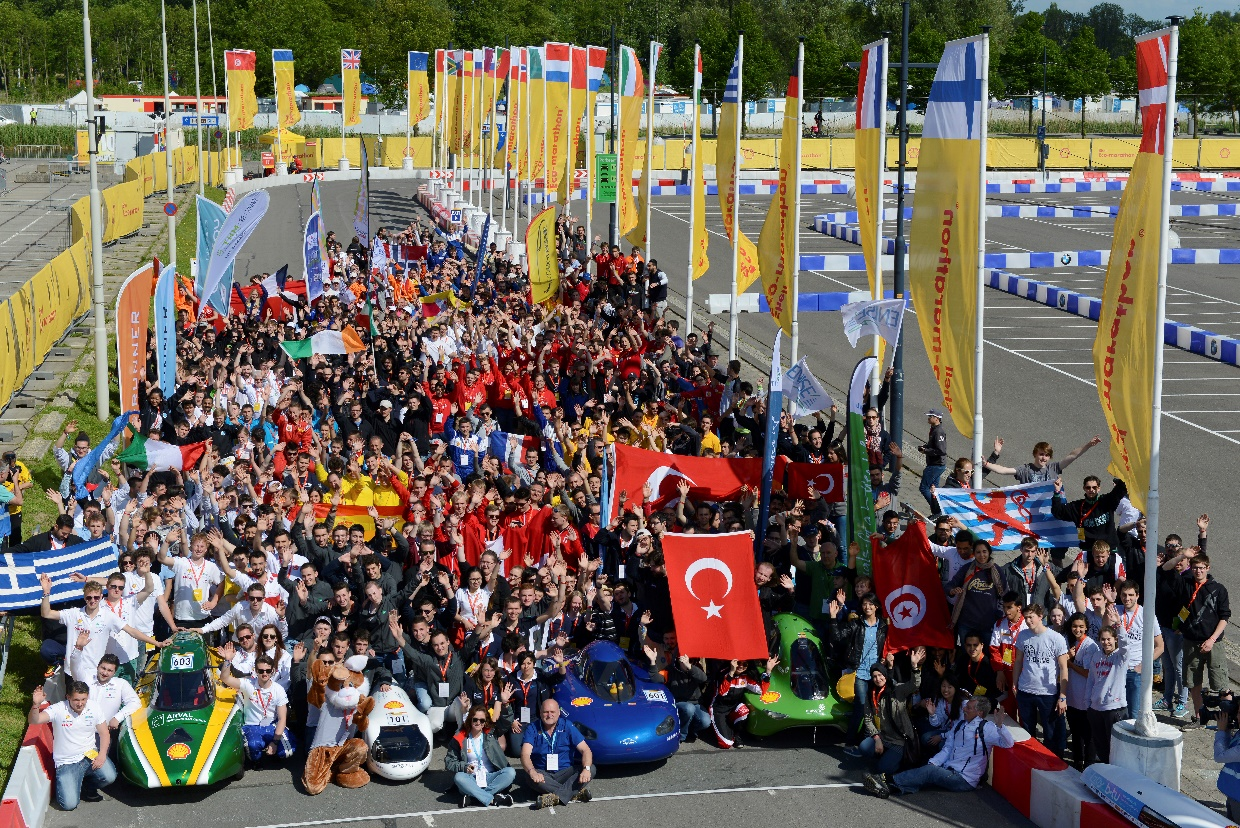
\includegraphics[scale=0.95]{foto1}
\caption{Family photo Shell Eco-Marathon 2015 Rotterdam}
\end{figure}

\begin{figure}
\hfill 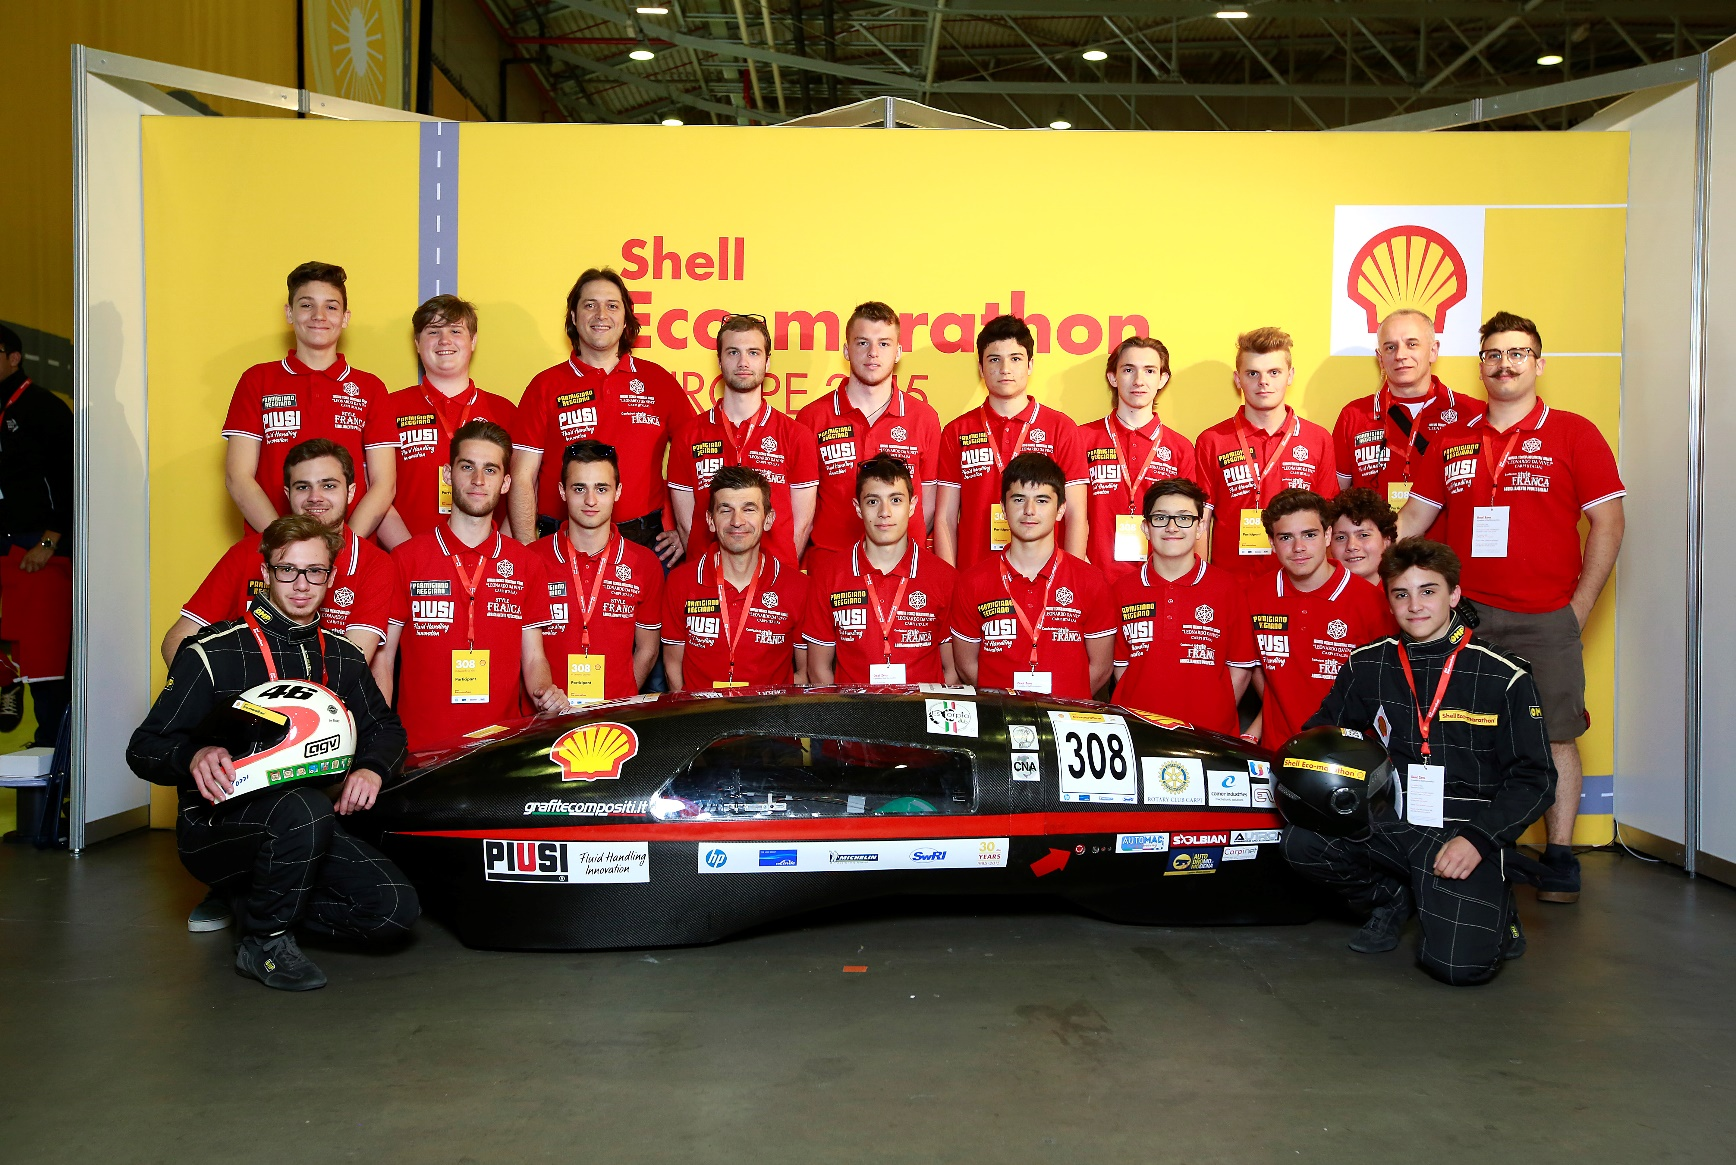
\includegraphics[scale=0.7]{foto2}
\caption{Team ZeroC ed Escorpio Evo alla Shell Eco-Marathon 2015}
\end{figure}
\newpage

\subsection{Obiettivo}
Descrizione obiettivo di questo lavoro
\newpage


\section{Il veicolo}
\subsection{Caratteristiche tecniche}
Descrizione delle caratteristiche del veicolo
\subsection{Modello matematico}
Descrizione del modello matematico fornito
\newpage


\section{Algoritmi genetici}
\subsection{Introduzione}
Un algoritmo genetico (GA) è un algoritmo di ricerca che trae ispirazione dalla genetica e dalla selezione naturale ed è spesso impiegato per la risoluzione di problemi di ottimizzazione. Le tecniche alla base dei GA permettono di simulare i processi di evoluzione presenti in natura, in particolare, il principio di sopravvivenza del più forte ispirato dalla teoria darwiniana. 

\subsection{Problema di ottimizzazione}

\subsection{Popolazione}
L'idea principale alla base di un GA è quella di creare una popolazione casuale di soluzioni, dette individui, e di farle evolvere in modo da trovare quella che risolve il problema dato in maniera ottima. Le caratteristiche di ogni individuo rappresentano il suo genoma, che può essere alterato in modo da trovare nuove soluzioni. La codifica più semplice per un genoma è quella binaria, dove ogni bit rappresenta una caratteristica dell'individuo. Sono possibili anche altre codifiche più complesse.

\subsection{Generazioni e fitness}
I GA sono algoritmi iterativi dove la popolazione iniziale viene fatta evolvere e ad ogni iterazione la nuova popolazione viene detta generazione.
Per compiere il processo evolutivo della popolazione e creare la nuova generazione, è necessario avere una misura di quanto una soluzione sia buona. Questa misura è detta fitness di un individuo. Maggiore è la fitness di un individuo, maggiore è la probabilità che l'individuo sopravviva e che i suoi geni possano creare nuovi individui in generazioni successive.

\subsection{Operatori genetici}
Gli operatori genetici sono un insieme di operazioni che vengono applicate ad ogni generazione per creare quella successiva.

\subsubsection{Selezione}
L'operatore di selezione è il primo operatore che viene applicato a ciascuna generazione. Questo operatore permette di scegliere quali individui della generazione corrente potranno riprodursi per creare i nuovi individui che faranno parte della generazione successiva.
Generalmente si selezionano gli individui con valori di fitness elevati.

Un caso particolare di selezione è l'elitismo, ovvero il mantenimento degli individui migliori di ciascuna generazione nelle generazioni successive. Questo tipo di selezione permette di non perdere le soluzioni migliori. Da un punto di vista biologico può essere visto proprio come la sopravvivenza del più forte.

\subsubsection{Crossover}

\subsubsection{Mutazione}

\subsection{Algoritmo base}

\subsection{Riproduzione degli schemi}

\subsection{Vantaggi}

\subsection{Problemi}
\newpage






\end{document}